% Source: test/pgfplots-sampled-bar-handlers.test.js, "log-ybar" case and
% its installed-PGFPlots rectangle/mark trace. The last spelling of each
% interval option wins: half-width bins centered at one quarter of the span.
% Reversed log2 x maps samples 1,2,8,16 to 8,6,2,0 cm. Three bars occupy
% x=[7,8], [4,6], [1,2] cm, with heights 1,2,4 cm. The fourth sample at
% (0,5) cm paints only a mark. Solid red marks separate all four from the
% teal fills and blue outlines. The gray rule is 0.18 cm below plot zero.
\documentclass[border=2pt]{standalone}
\usepackage{pgfplots}
\pgfplotsset{compat=1.18}
\begin{document}
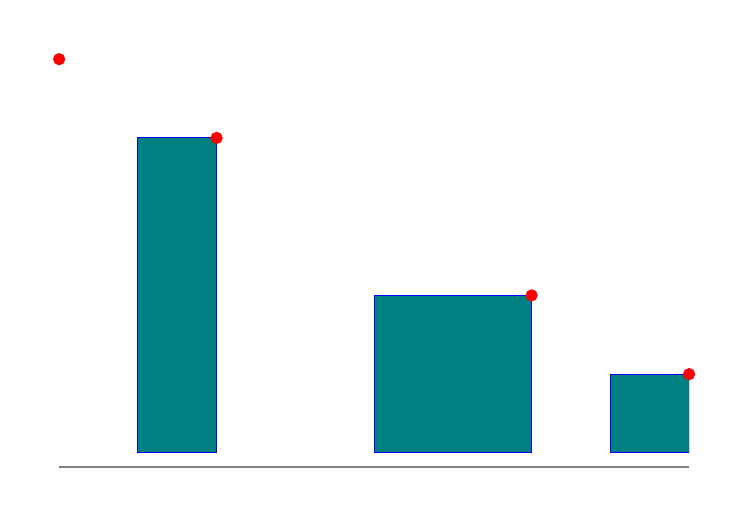
\begin{tikzpicture}
  \path[use as bounding box] (-0.4,-0.4) rectangle (8.4,5.4);
  \draw[gray] (0,-0.18) -- (8,-0.18);
  \begin{axis}[hide axis,scale only axis,at={(0,0)},anchor=south west,
    width=8cm,height=5cm,enlargelimits=false,
    xmode=log,log basis x=2,x dir=reverse,xmin=1,xmax=16,ymin=0,ymax=5]
    \addplot[draw=blue,fill=teal,mark=*,mark size=2pt,mark options={draw=red,fill=red},
      /tikz/ybar interval,bar interval width=0.8,/pgf/bar interval width=0.5,
      /pgf/bar interval shift=0.6,bar interval shift=0.25,samples at={0,1,3,4}]
      ({2^x},{x+1});
  \end{axis}
\end{tikzpicture}
\end{document}
